\def\longueurVecteurs{1.75}
\def\interSpace{0.5}
\def\interSpaceY{2}

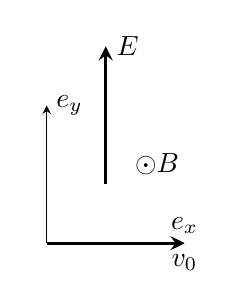
\begin{tikzpicture}
  \tikzstyle{fleche}=[->,>=stealth];
  \draw [fleche] (0,0) -- (\longueurVecteurs,0) node [above] {$\vv{e_x}$};
  \draw [fleche] (0,0) -- (0,\longueurVecteurs) node [right] {$\vv{e_y}$}; 
  \draw [fleche, very thick,\JRLblue] (0,0) -- (0:\longueurVecteurs) node [below] {$\vv{v}_0$};
  \draw [fleche, very thick,\JRLred] (0.75,0.75) -- (0.75,0.75+\longueurVecteurs) node [right] {$\vv{E}$};
  %\draw [fleche] (\longueurVecteurs/2,0) arc (0:45:\longueurVecteurs/2) node [midway,right] {$\alpha$}; 
  \draw (1,1) node [right] {$\odot \vv{B}$};
  \draw (0,0) node[below left]{$\ptO$};

\end{tikzpicture}
